% PAKETE UND DOKUMENTKONFIGURATION
\documentclass[11pt, a4paper]{article}

% Encoding für Umlaute
\usepackage[utf8]{inputenc}
\usepackage[T1]{fontenc}

% Silbentrennung
\usepackage[english]{babel}

% erweiterte Matheumgebungen und Formelnummer mit Sectionnummer
\usepackage{amsmath}
\numberwithin{equation}{section}

% Braket Notation
\usepackage{braket}
\usepackage{isotope}

% zusätzliche mathematische Schriftarten
\usepackage{amsfonts}

% verschiedene mathematische Symbole
\usepackage{amssymb}

% Einheiten setzen z.B. \SI{10}{\kilo\gram\meter\per\second\squared}
% Fehler: \SI{10 +- 0,2e-4}{\metre}
\usepackage{siunitx}
\sisetup{
  separate-uncertainty
}

% Einheitendefinitionen
\DeclareSIUnit{\skt}{Skt.}
\DeclareSIUnit{\gauss}{G}

% Operatordefinitionen
\DeclareMathOperator{\erf}{erf}

% Randbreiten
\usepackage[left=3.5cm,right=3.5cm,top=3cm,bottom=3cm,twoside]{geometry}

% Bilder einfügen
\usepackage{graphicx}

% Verweise innerhalb des Dokuments
\usepackage{hyperref}
\hypersetup{
	colorlinks = true,
	allcolors = {black}
}

% bessere Tabellenlayouts
\usepackage{booktabs}
\usepackage{multirow}
\usepackage{multicol}

% Seitenlayout (Kopfzeile)
\usepackage{fancyhdr}

% Float Barriers
\usepackage{placeins}

% Pakete für gedrehte Subfigures
\usepackage{caption}
\usepackage{subcaption}
\usepackage{rotating}

% Paket für textumflossene Abbildungen und Tabellen
\usepackage{wrapfig}

\usepackage{float}

% Caption-Setup
\captionsetup{font={small}}
\renewcommand{\thefigure}{\thesection.\arabic{figure}}
\renewcommand{\thesubfigure}{\alph{subfigure}}
\renewcommand{\thetable}{\thesection.\arabic{table}}
\renewcommand{\thesubtable}{\alph{subtable}}

% Manuelle Silbentrennung
\hyphenation{Re-so-na-tor Mo-den-ab-stand Re-so-na-tor-län-ge Spek-t-ro-me-ter}

% Tiefe des Inhaltsverzeichnisses (Level: 1 sections, 2 subsections,
% 3 subsubsections)
\setcounter{tocdepth}{3}

% FANCYHDR SETUP
\pagestyle{fancy}
\fancyhead[EL,OR]{\thepage}
\fancyhead[ER]{\leftmark}
\fancyhead[OL]{\rightmark}

\renewcommand{\sectionmark}[1]{
\markboth{\thesection{} #1}{\thesection{} #1}
}
\renewcommand{\subsectionmark}[1]{
\markright{\thesubsection{} #1}
}

% DOKUMENTINFORMATIONEN
\title{Pi in the Sky\\Orbit Determination of 2004 BL86}

\author{Christopher Deutsch\footnote{christopher.deutsch@uni-bonn.de} \and Christian Bespin\footnote{christian.bespin@uni-bonn.de}}

\date{\today}

\begin{document}

\begin{titlepage}

\maketitle

% DURCHFÜHRUNGSDATUM UND TUTOR
\begin{center}
\begin{tabular}{l r}
Execution: & May 25/26, 2015 \\
Group: & $\alpha$ 6 \\
Tutor: & Rui Zhang
\end{tabular}
\end{center}

% ZUSAMMENFASSUNG
\begin{abstract}
\noindent 
This report shall be concerned with determining the orbital parameters of the asteroid 2004 B86 from terestial observation with the Pi in the Sky telescope in Chile.
\end{abstract}

\end{titlepage}

% INHALTSVERZEICHNIS
\tableofcontents
% Neue Seite nach TOC
\newpage

% INHALT VERSUCHSPROTOKOLL

\section{Introduction}
In the night of January 26/27, 2015 a near-earth approach of the asteroid 2004 BL86 took place and was observed with the telescope \emph{Pi in the Sky} in Chile, San Pedro de Atacama.
The asteroid was visible on more than a thousand photos, which where shot from 3:10 to 6:30 UT.
After some preprocessing of the collected images the position of the asteroid could be determined using stationary reference stars.

\section{Theory}

\subsection{Kepler's Laws}
The bound motion of an object in a potential of the form:
\begin{align}
	V \propto \frac{1}{r}
\end{align}
where $r$ is the distance from the field source, is described by \emph{Kepler's Laws}.
In the case of astronomy, an object (e.g.\ planets, asteroids) is bound by the gravitational attraction of a central body and its orbit obeys the three Kepler's laws of planetary motion:
\begin{enumerate}
	\item The bound orbit of an object around a central body is described by an ellipse, where the position of the central body coincides with one of the two foci of the ellipse.
	
	\item Since the torque of the central body on the orbiting one is zero, angular momentum is conserved. As a result the angular velocity of the orbiting body increases as its distance to the central body decreases.
	More precisely a line joining the orbiting body and the central body sweeps out equal areas in equal time intervals.
	
	\item The revolution period $T$ squared divided by the semi-major axis $a$ cubed is constant for a given central body.
	Therefore one can calculate the revolution period of a planet only knowing the length of its semi-major axis and the ratio $T^2/a^3$ for an arbitrary object in the same potential:
	\begin{align}
		\frac{T_1^2}{a_1^3} = \frac{T_2^2}{a_2^3}
	\end{align}
\end{enumerate}

\subsection{Equatorial Coordinate System}
\begin{figure}[h]
	\centering
	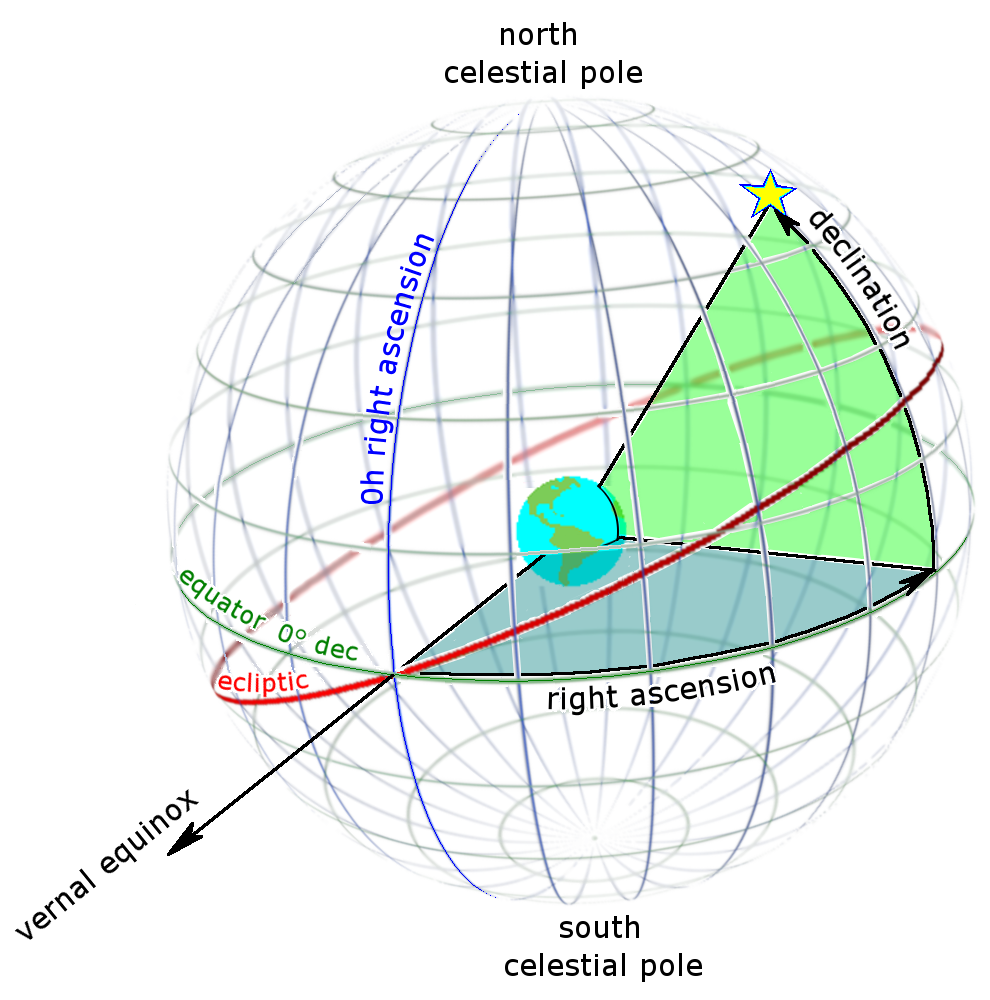
\includegraphics[width=0.7\textwidth]{./figures/equatorial_cs.png}
	\caption{Illustration explaining the equatorial coordinate system in astronomy. Credit: \url{https://commons.wikimedia.org/wiki/File:Ra_and_dec_on_celestial_sphere.png}}
\end{figure}
The equatorial coordinate system is an astronomical coordinate system using earth's equator as its reference plane as opposed to the ecliptic coordinate system using the ecliptic for reference.
The position of an object on the celestial sphere is then defined with two angles $\alpha$ and $\delta$.
The declination~$\delta$ measures the height of the object from the celestial equator (projection of earth's equator on the celestial sphere), where the north celestial pole has declination $+\SI{90}{\degree}$.
The right ascension $\alpha$ is the angular distance of the object's projection on the equator plane to the vernal equinox, which is the intersection of ecliptic and equatorial plane.
It is because of this reference point, that the equatorial coordinate system is independent of earth's rotation.

\subsection{Orbital Elements}
\label{sec:orbital_elements}
\begin{figure}[h]
	\centering
	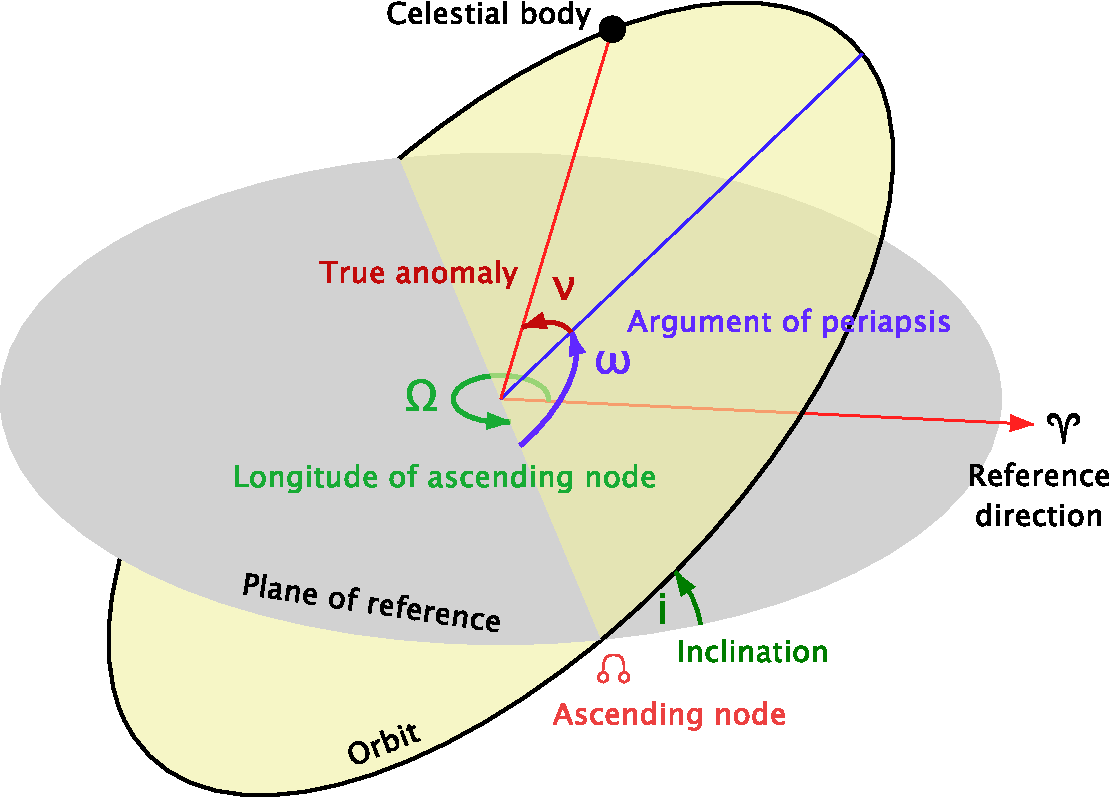
\includegraphics[width=0.75\textwidth]{./figures/orbital_elements.pdf}
	\caption{Illustration of the classical orbital elements of an arbitrary celestial body. Credit: \url{https://en.wikipedia.org/wiki/File:Orbit1.svg}}
\end{figure}
The position of a body on an ellipse can be described with the so called orbital elements which are a set of parameters to identify a specific orbit.
For astronomical purposes those parameters are chosen as the so called Keplerian elements given as:
\begin{itemize}
	\item $a$: length of the semimajor axis of the ellipse	
	\item $e$: eccentricity of the ellipse	
	\item $i$: inclination	
	\item $\Omega$: right ascension of the ascending node	
	\item $\omega$: angular distance of the periapsis from the ascending node	
	\item $\nu$: true anomaly defining the position of the orbiting body at a certain point in time
\end{itemize}
An orbiting body can be identified by those parameters which are given in a coordinate system with its origin in the center of the ellipse and relative to a reference plane and direction.
While the first five values define time-independent size and orientation of the orbit, the anomaly is a function of time and leads to the position of the body on the orbit.
For a given time it is necessary to know six parameters to describe an orbit and distinguish between different orbits because of the six degrees of freedom for orbit determination.
They correspond to three spacial dimensions and the respective velocities which can also be used for orbit identification.

\section{Analysis}

\subsection{Description}
We were given the measurement data of the approach.
Each data point containing UT time $t$ of the beginning of exposure, declination $\delta$ and right ascension $\alpha$ of the asteroid as measured at the observatory location in Chile: 
\begin{itemize}
	\item longitude: \SI{-68.18000000}{\degree}
	\item latitude: \SI{-22.95332778}{\degree}
	\item altitude: \SI{2430}{\meter}
\end{itemize}

\subsection{Idea}
Due to the lack of time and resources the usual methods of orbit determination were unfeasible.
Therefore we tried to find a simpler method of orbit determination based on a least-squares fit.
Our method involved the following steps:
\begin{enumerate}
	\item \textbf{Hypothesis of the asteroid's orbit:}\\
	Guess the approximate orbital elements (c.f.\ \ref{sec:orbital_elements}) of the asteroid's orbit, which will be refined in the following steps.
	
	\item \textbf{Position of the asteroid at time of observation:}\\
	From the (guessed) orbital elements the asteroids trajectory at the time of observation can be calculated.
	
	\item \textbf{Determining observatory location in sun's coordinate system:}\\
	Using literature values for the orbital elements the position of earth can be determined at the time of observation.
	Moreover the location of the observatory on earth has to be considered.
	Using the longitude, latitude and altitude of the observatory and the position of earth, the observation location in the coordinate system of the sun can be determined.
	
	\item \textbf{Calculation of the observation angles of the hypothetical asteroid:}\\
	The hypothesis of the asteroid's orbit and the determined location of the observatory in sun's coordinate system allows us to calculate the angles $\alpha$ and $\delta$ at which the asteroid appears on the celestial sphere. In the next step will improve on the hypothesis using a least-squares fit to the observed trajectory.
	
	\item \textbf{Fitting of the orbital elements to the observed trajectory on the celestial sphere:}\\
	We improve on the hypothesis of the asteroid's orbit by using a least-squares fit (via orbital elements of the asteroid) to the observational data. Using this method it is imperative that a good guess of the asteroid's orbit has to be made.	
\end{enumerate}



\subsection{Correction of Exposure Time}
The given UT time $t$ measured the start of the exposure time of length \SI{10}{s}.
To determine the effective time $t^*$ of measurement, half the exposure time has to be added:
\begin{align}
	t^* = t + \SI{5}{s}
\end{align}

\subsection{Transforming of Coordinates}
As a first approach, earth's position in the equatorial coordinate frame at observation time is reconstructed.
Since all Keplerian elements but true anomaly are not dependent on time they can be looked up, see for example in \emph{Earth Fact Sheet}\footnote{http://nssdc.gsfc.nasa.gov/planetary/factsheet/earthfact.html}.
True anomaly itself can not be easily computed so we did a linear approximation based on the data \emph{Wolfram Alpha}\footnote{e.g. http://www.wolframalpha.com/input/?i=true+anomaly+earth+01-26-2015} gives for the time period of observation which is short compared to earth's revolution time so that a linear approximation for $\nu(t)$ should be sufficient for our needs.

Second, the observatory's position on earth is taken into account.
Based on the given location, altitude and in the used reference frame it can be easily computed in spherical coordinates.
After transforming both earth's position (to be precise the position of the center of the earth) from Keplerian elements and the obersavtory's position from spherical to spacial coordinates and velocity the time-dependent state vector of the observer can be calculated.
This is done with the Python module \emph{poliastro}.

\subsection{?}
Hypothesis of asteroid parameters for fit\\
In order to propagate  a given state vector along an orbit it is necessary to solve Kepler's equation
\begin{align}
	M = E - e\, \sin E
\end{align}
(M: mean anomaly, E: eccentric anomaly, e: eccentricity).
While eccentricity is a orbit parameter, $M$ is often chosen as an orbital element and is, as eccentric anomaly, connected with true anomaly while all of them can be used to determine a body's position on an orbit.
There are multiple ways of numerically solving Kepler's equation in order to find the true anomaly where findig the eccentric anomaly as root of the equation is one of these alongside a way using Banach fixed-point theorem.
True anomaly can then be calculated with
\begin{align}
\cos\nu = \frac{\cos E - e}{1 - e \cos E}
\end{align}
Again the \emph{poliastro} package is used for this task as it offers a convenient function to propagate the body's position for a given time $t$ based on the current state vector.

Determining observation angles (on earth) from asteroid position\\
Minimizing $\chi^2$




\section{Conclusion}


\FloatBarrier
% BIBLIOGRAPHIE
\vspace{\fill}
% Maximale Anzahl der Einträge in Klammer
% Zitieren mit \cite{lamport94}
\begin{thebibliography}{19}

\bibitem{krane}
	Kenneth S. Krane,
	\emph{Introductory Nuclear Physics},
	John Wiley \& Sons 1988

\end{thebibliography}

% APPENDIX
\begin{appendix}
\section{Appendix}

\end{appendix}

\end{document}
